\section{Inequalities with Absolute Value and Quadratic Functions}

\begin{definition}[Graphical Interpretation of Equations and Inequalities]
    Suppose $f$ and $g$ are functions.
    \begin{itemize}
        \item The solutions to $f(x)=g(x)$ are the $x$ values where the graphs of $y=f(x)$ and $y=g(x)$ \textit{intersect}.
        \item The solutions to $f(x)<g(x)$ are the $x$ values where the graphs of $y=f(x)$ is \textit{below} the graph of $y=g(x)$.
        \item The solutions to $f(x)\geq g(x)$ are the $x$ values where the graphs of $y=f(x)$ is \textit{above} the graph of $y=g(x)$.
    \end{itemize}
\end{definition}

\begin{definition}[Inequalities Involving the Absolute Value]
    Let $c$ be a real number.
    \begin{itemize}
        \item For $c>0$, $|x|<c$ is equivalent to $-c < x < c$.
        \item For $c>0$, $|x|\leq c$ is equivalent to $-c \leq x \leq c$.
        \item For $c \leq 0$, $|x|<c$ has no solution, and for $c < 0$, $|x| \leq c$ has no solution.
        \item For $c\geq 0$, $|x| > c$ is equivalent to $x<-c \cup x>c$.
        \item For $c\geq 0$, $|x| \geq c$ is equivalent to $x\leq -c \cup x \geq c$.
        \item For $c < 0$, $|x| > c$ and $|x| \geq c$ are true for all real numbers.
    \end{itemize}
\end{definition}

\subsection{Exercises}
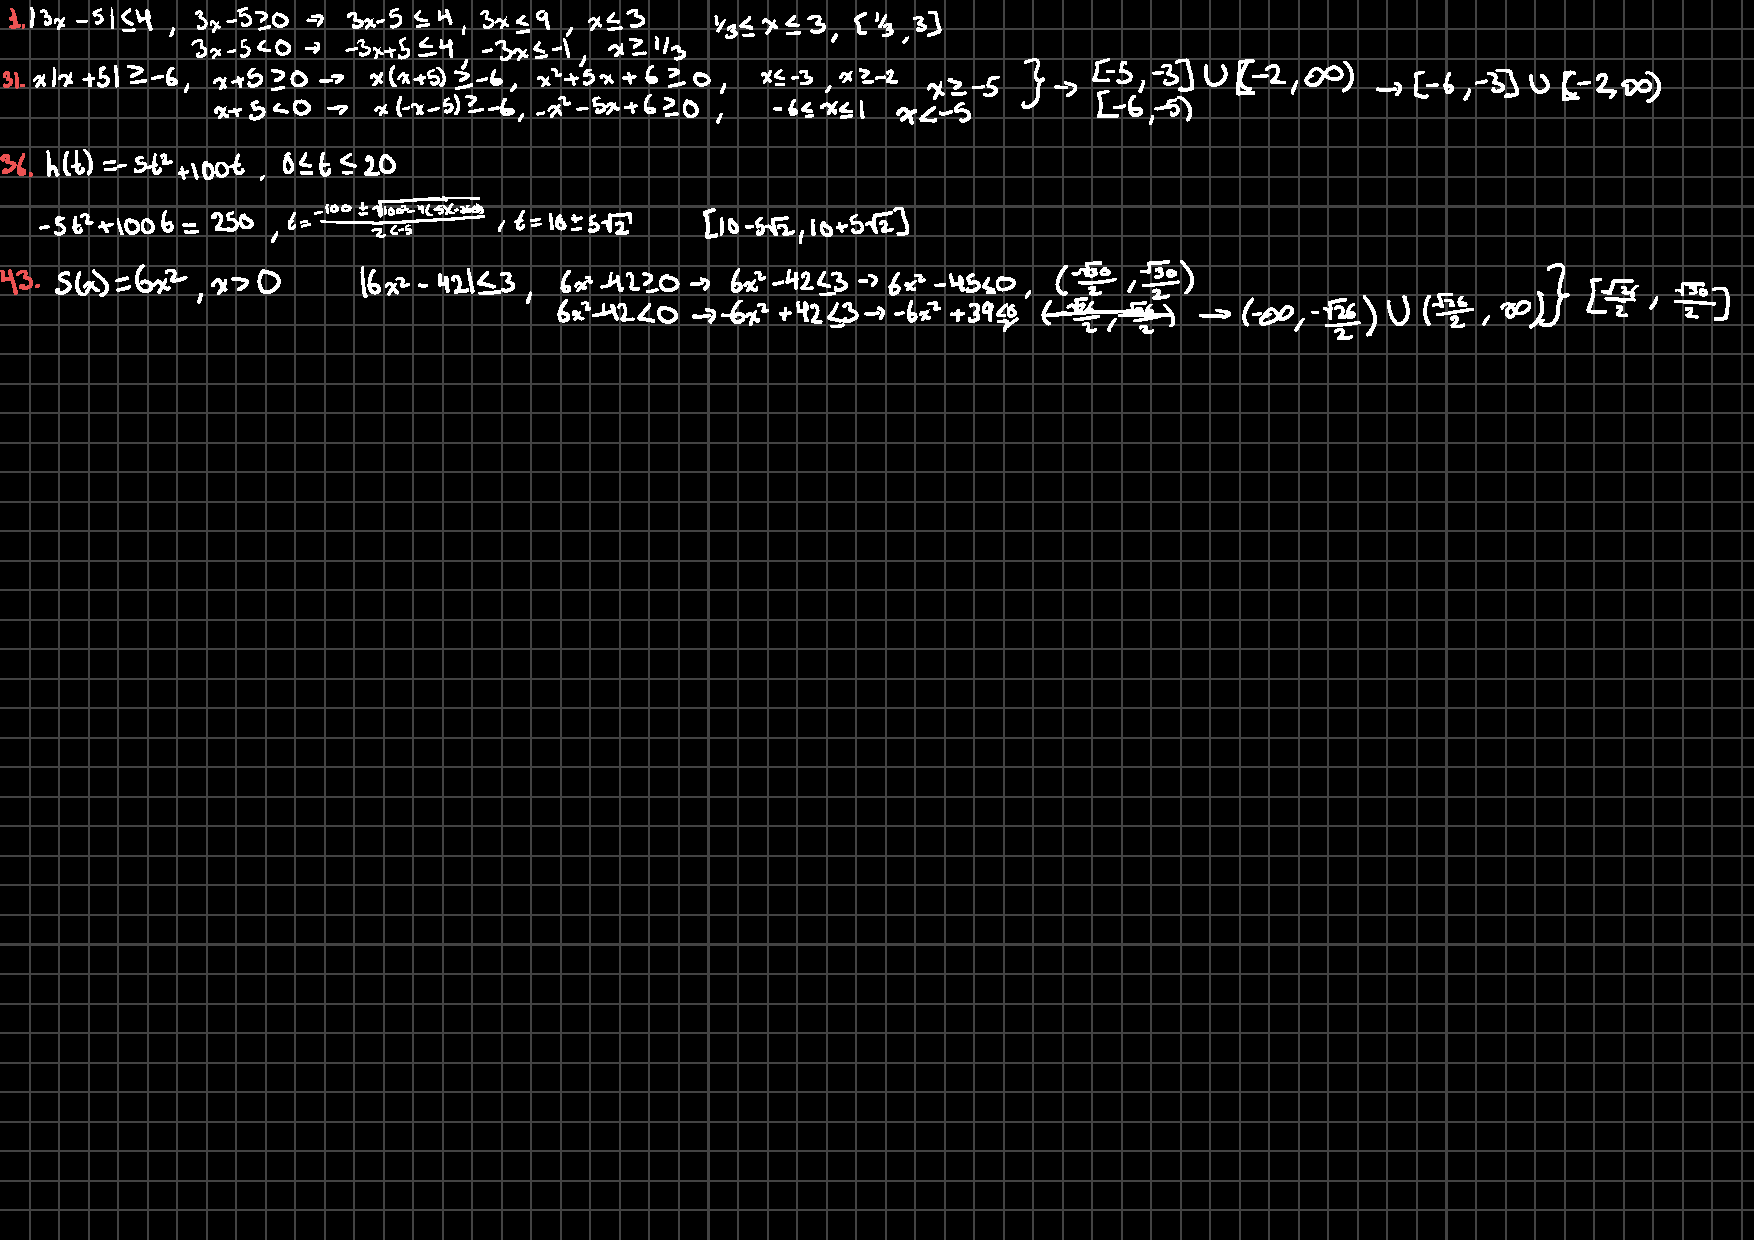
\includepdf[pages=-]{Exercises/02/04.pdf}